\section{Einsatz von Bypassdioden}

\subsection{Gründe für Einsatz von Bypassdioden}
\begin{enumerate}
    \item Vermeidung von Überhitzung verschatteter Zellen (Hotspots)
    \item Leistungssteigerung indem sichergestellt wird, dass bei Verschattung eines Moduls nicht der gesamte String beeinträchtigt wird. (Modul bzw. Zelle wird "übersprungen")
\end{enumerate}



\subsection{Solarmodul ohne Bypassdioden}
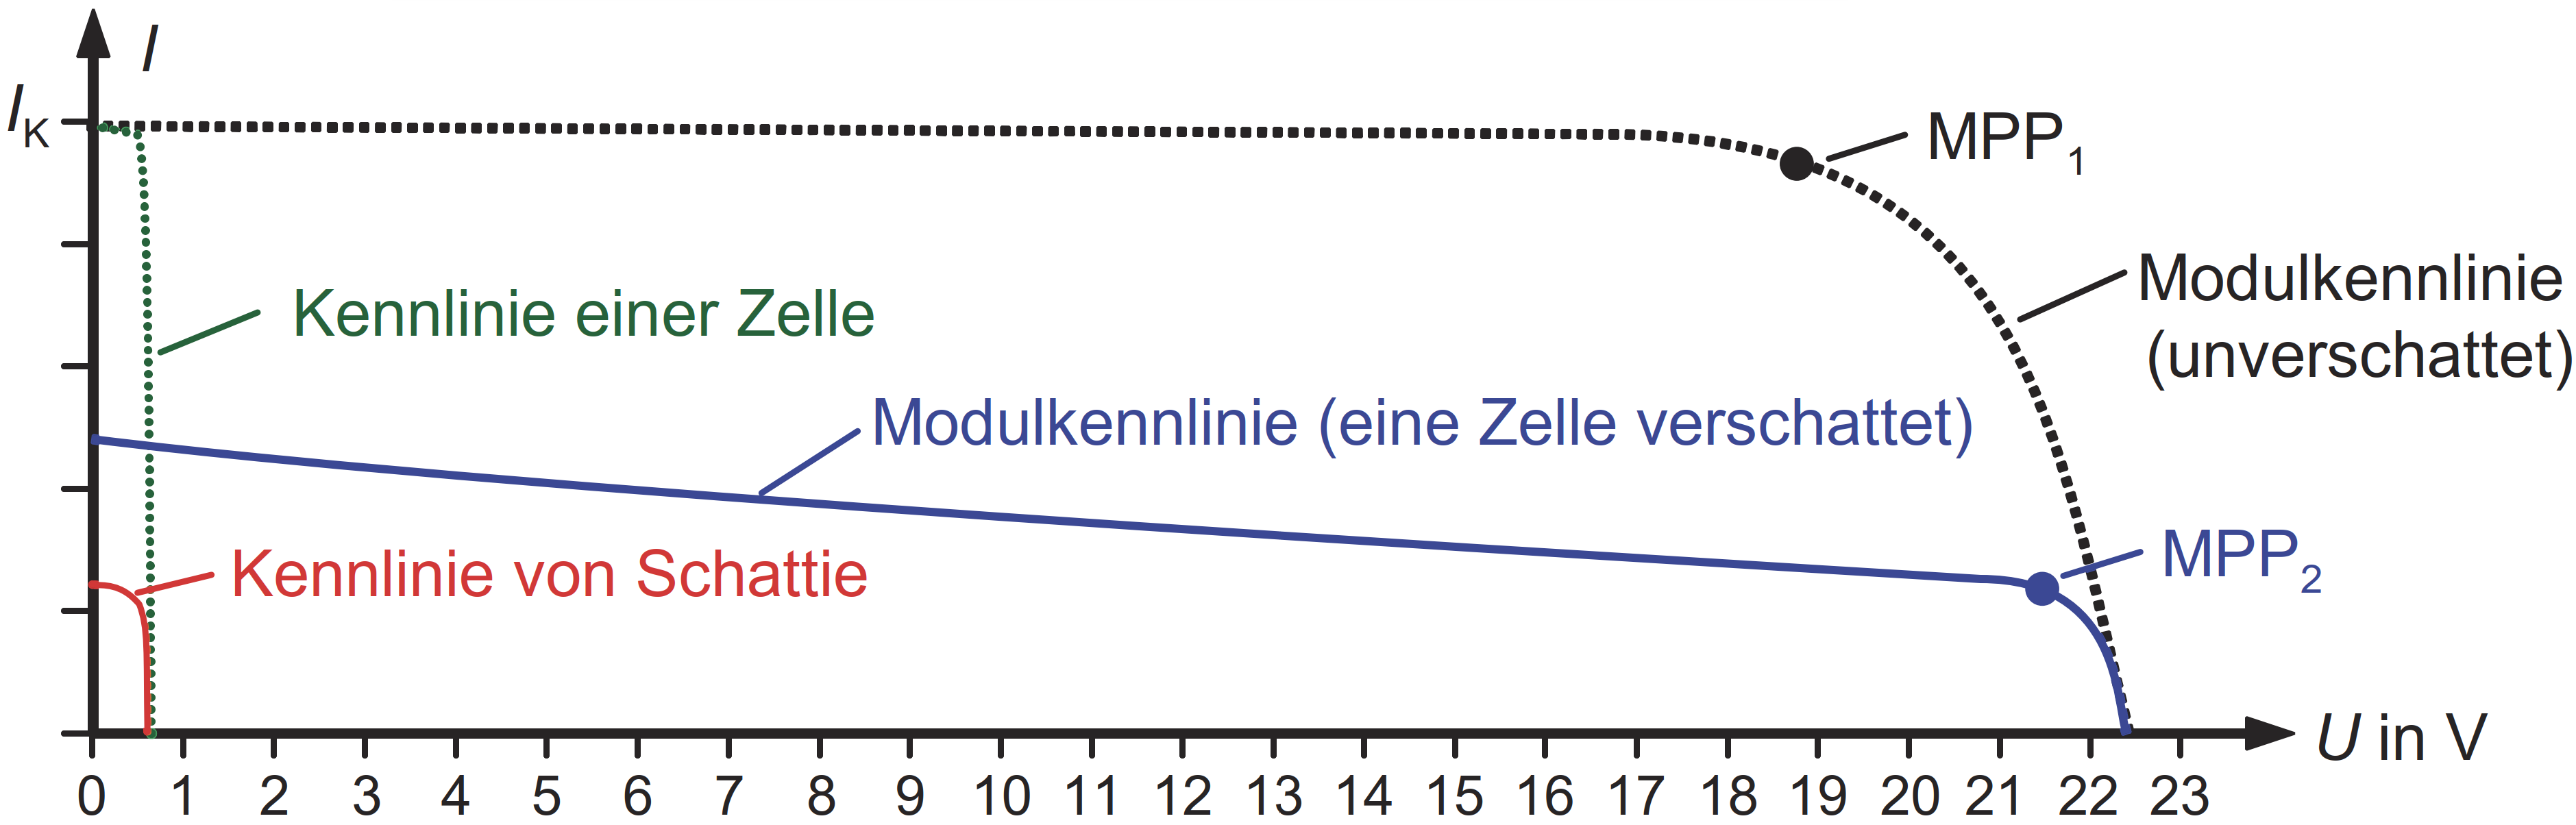
\includegraphics[width=0.95\columnwidth]{images/Verschattungsverluste_ohne_Bypassdiode.png}



\subsection{Solarmodul mit Bypassdioden}
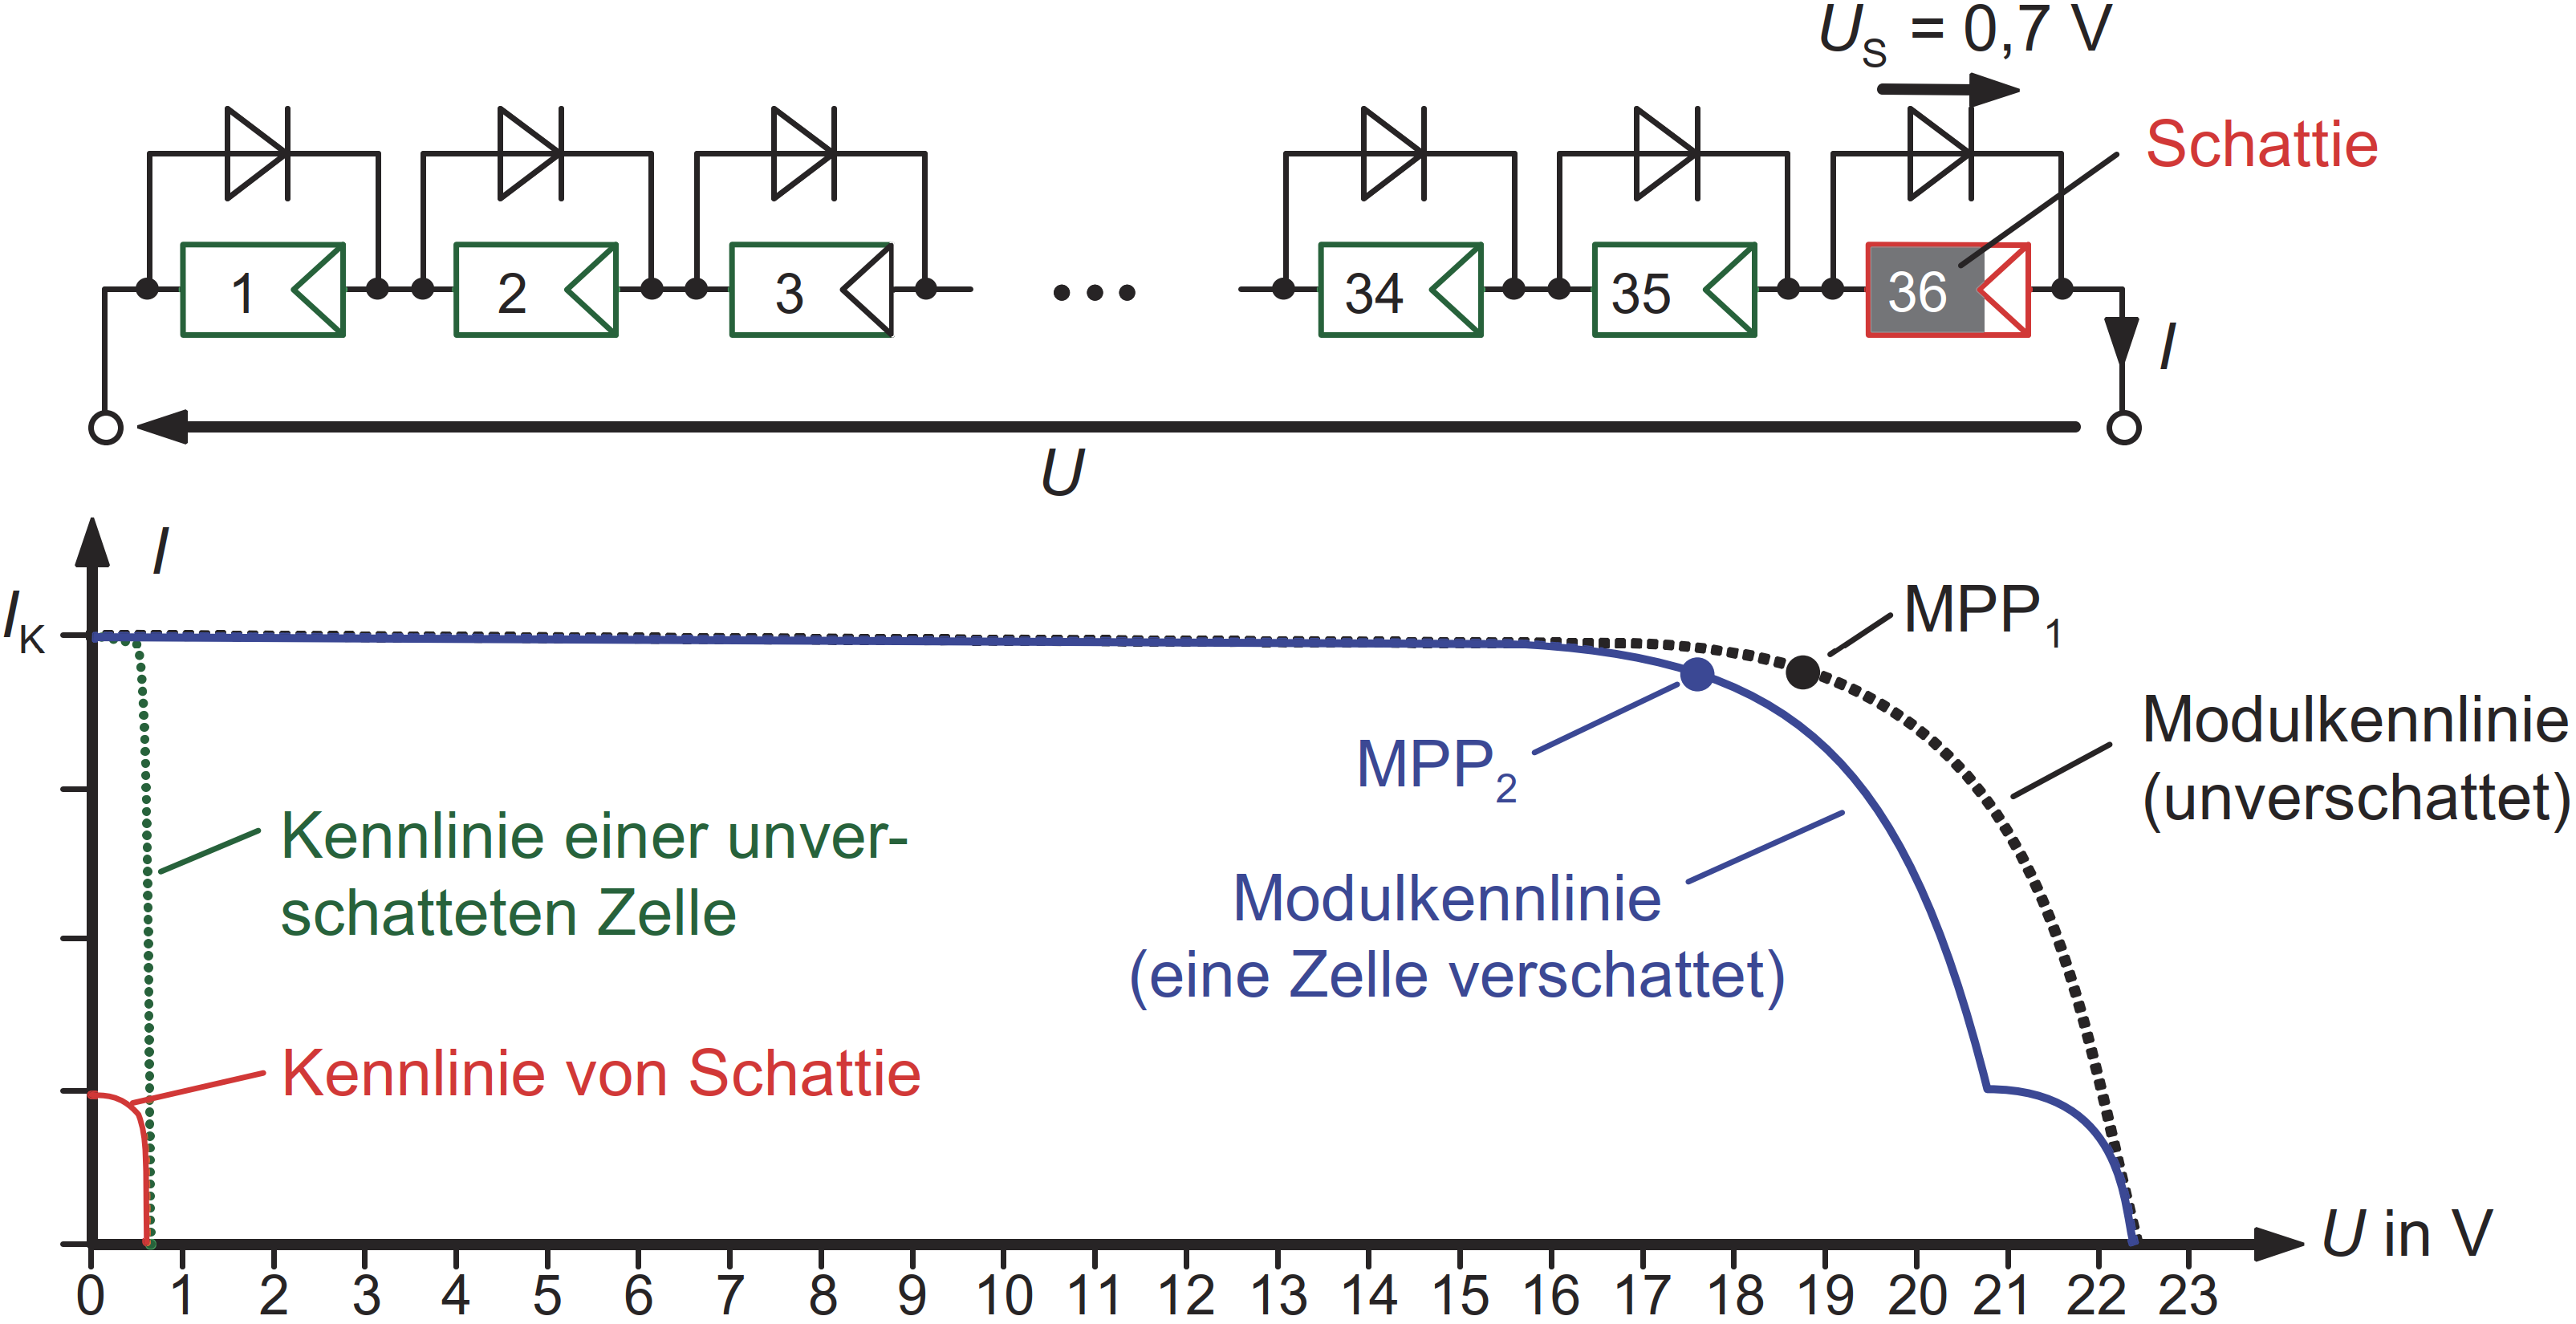
\includegraphics[width=0.95\columnwidth]{images/Verschattungsverluste_mit_Bypassdiode.png}



\subsection{Auswirkung Anzahl Bypassdioden}
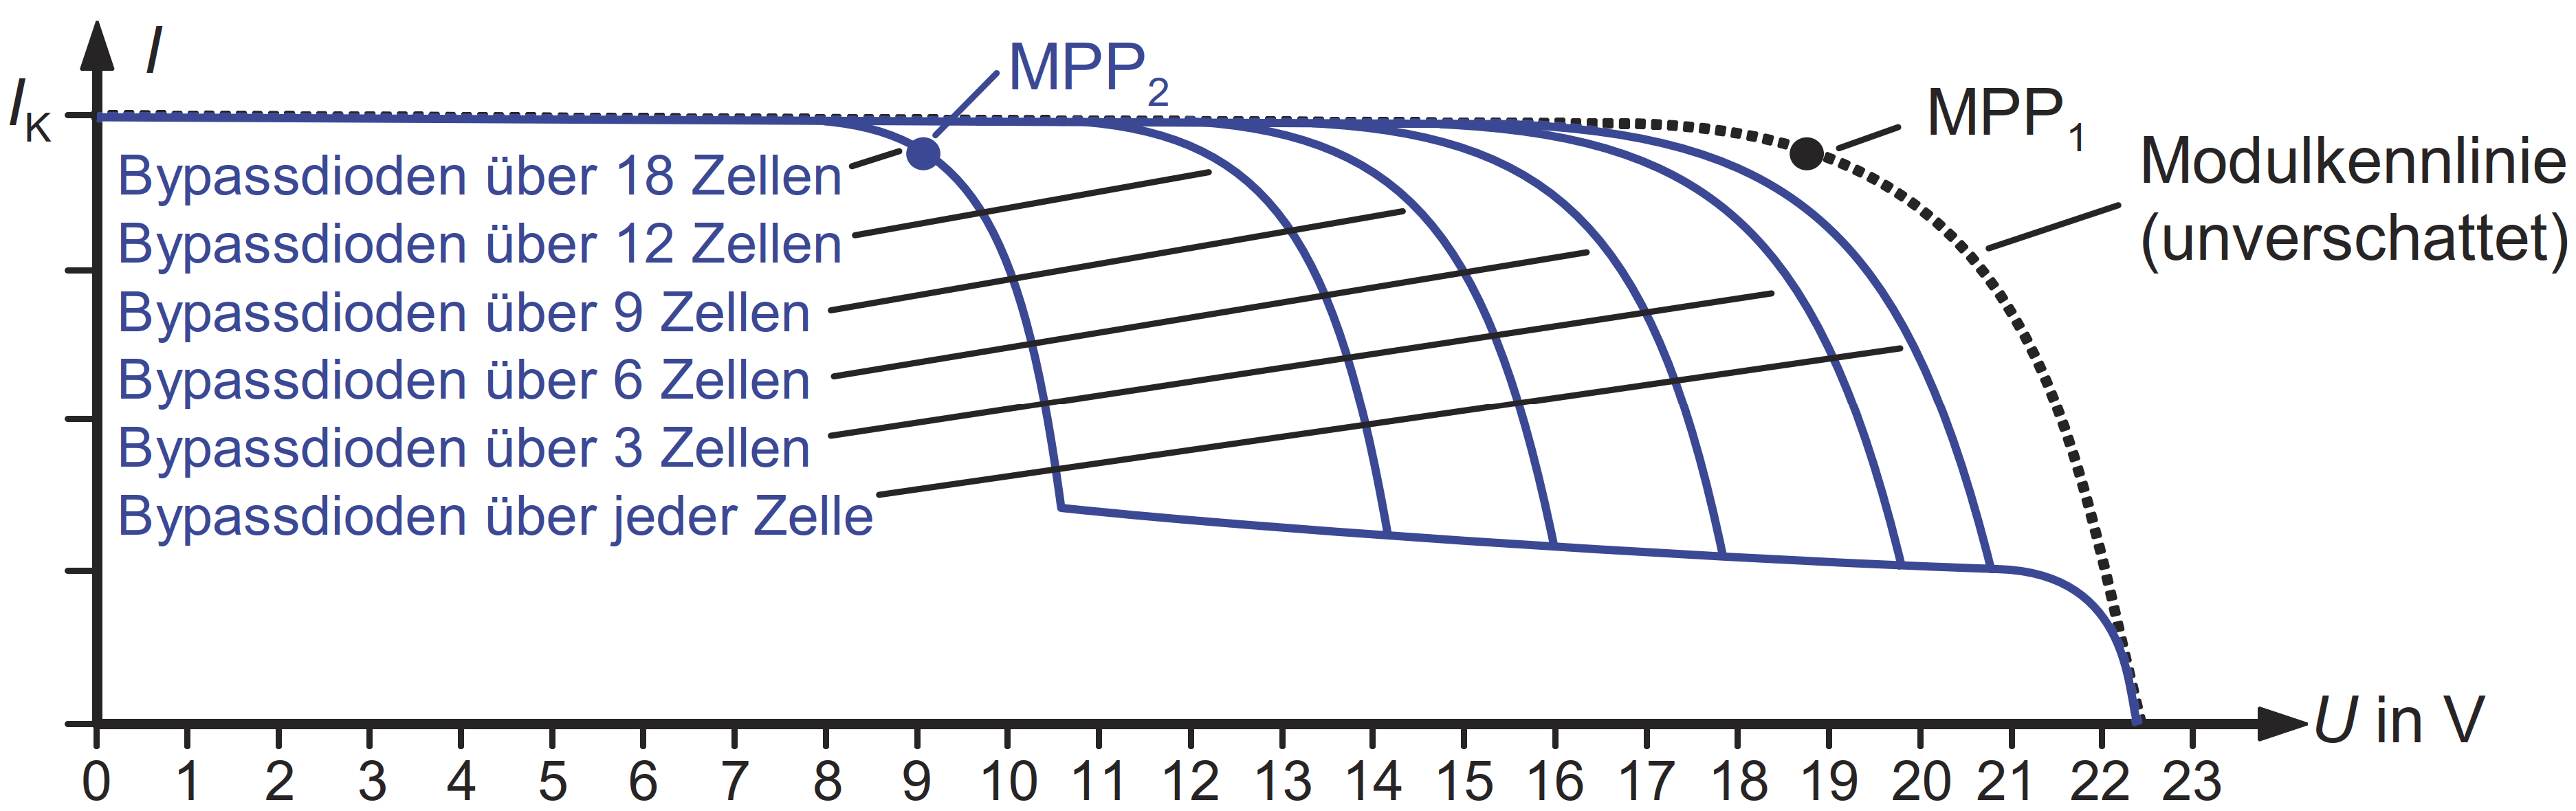
\includegraphics[width=0.95\columnwidth]{images/Reduzierung_Verschattungsverluste_durch_Bypassdioden.png}


\subsection{Vermeidung von Hotspots durch Bypassdioden}
\subsubsection{Solarmodul ohne Bypassdioden}
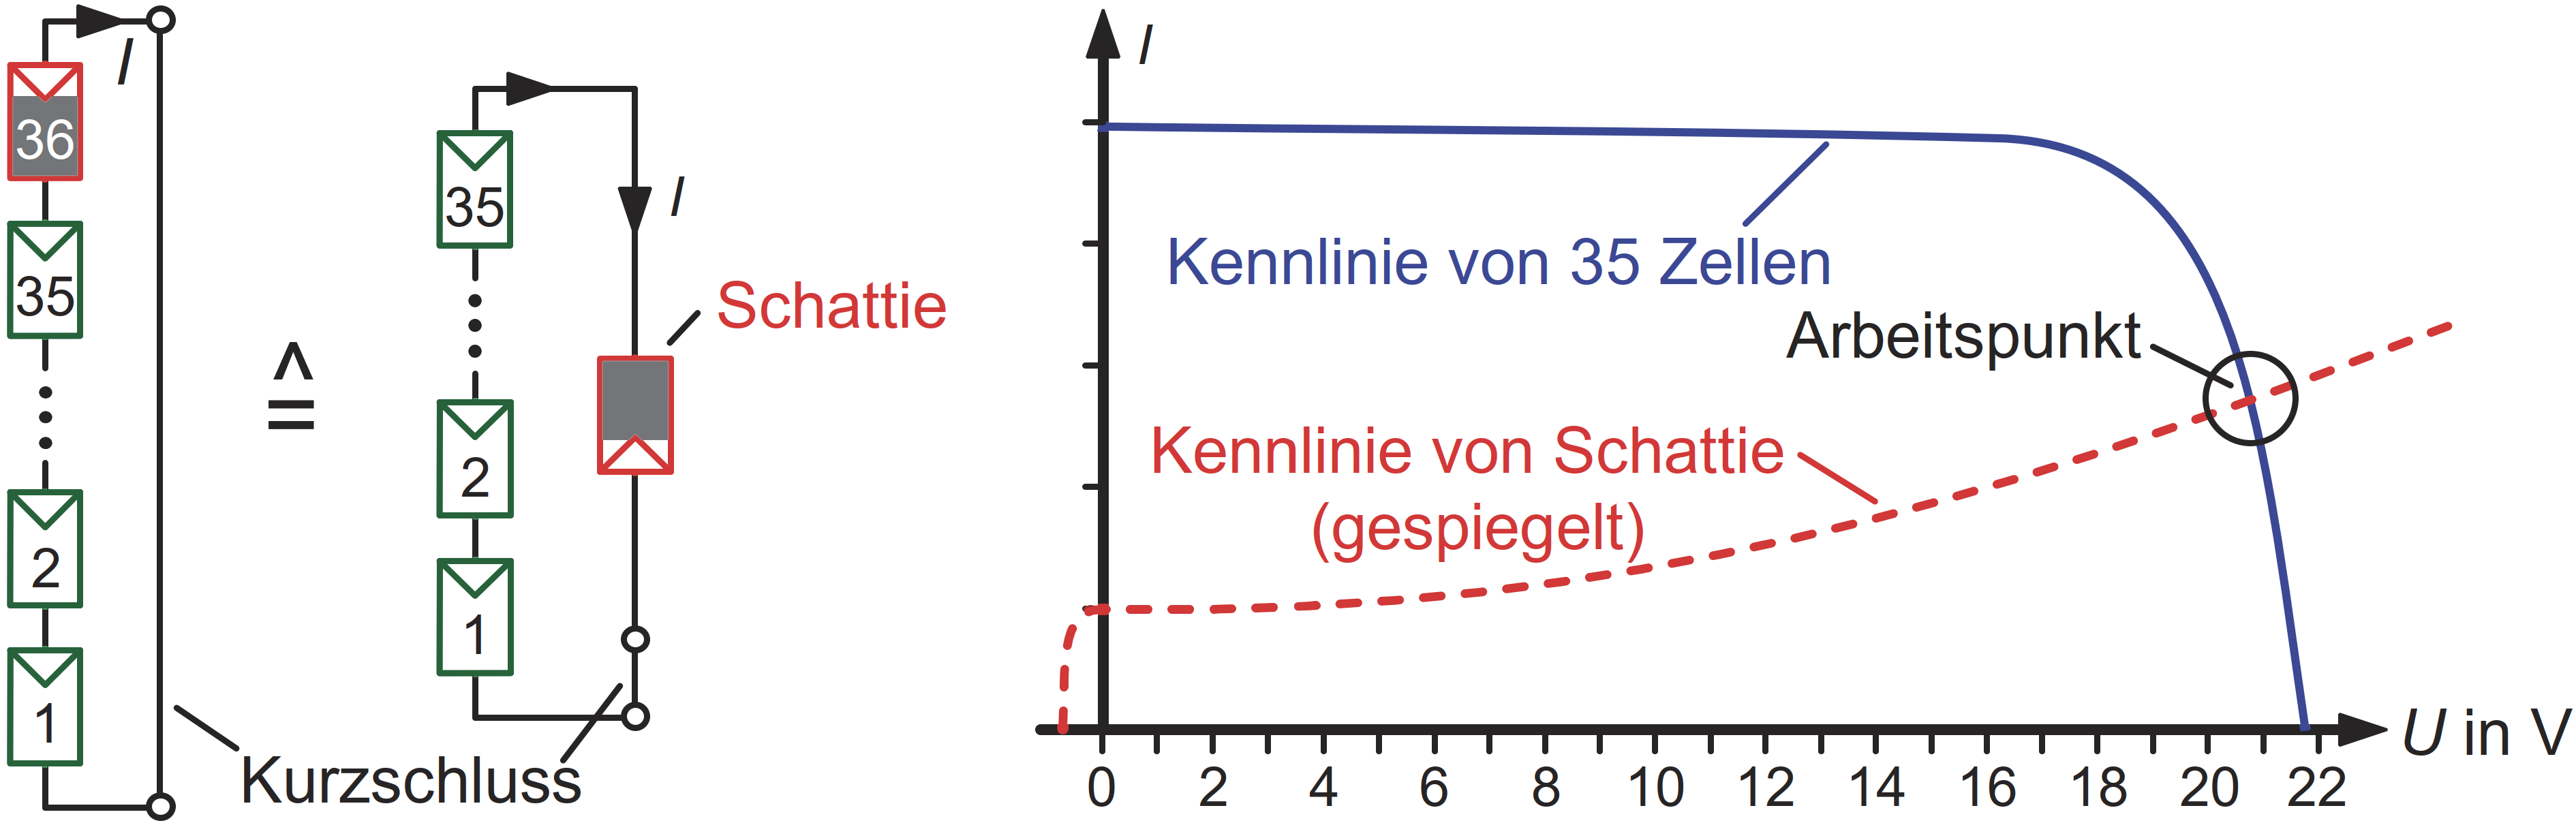
\includegraphics[width=0.95\columnwidth]{images/Vermeidung_von_Hotspots_1.png}



\subsubsection{Solarmodul mit 2 Bypassdioden}
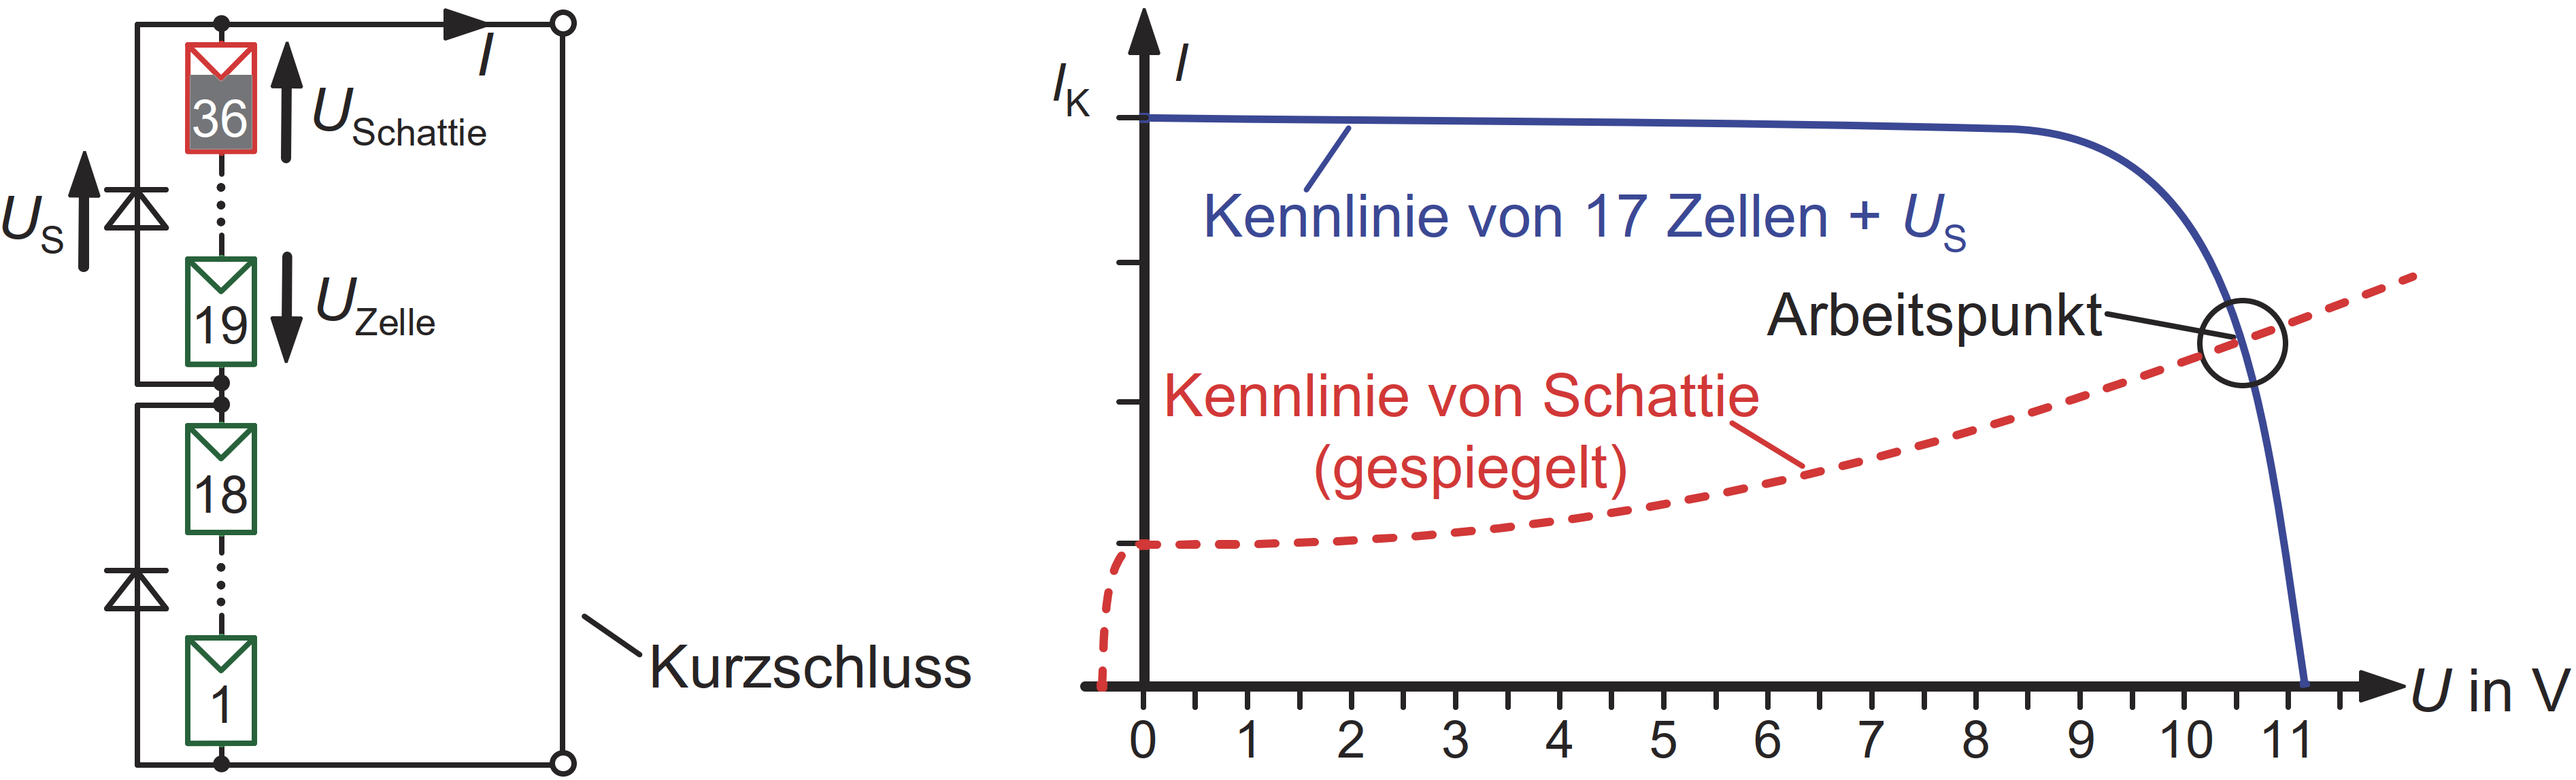
\includegraphics[width=0.95\columnwidth]{images/Vermeidung_von_Hotspots_2.png}



\subsubsection{Betrachtung verschiedener Verschattungsgrade}
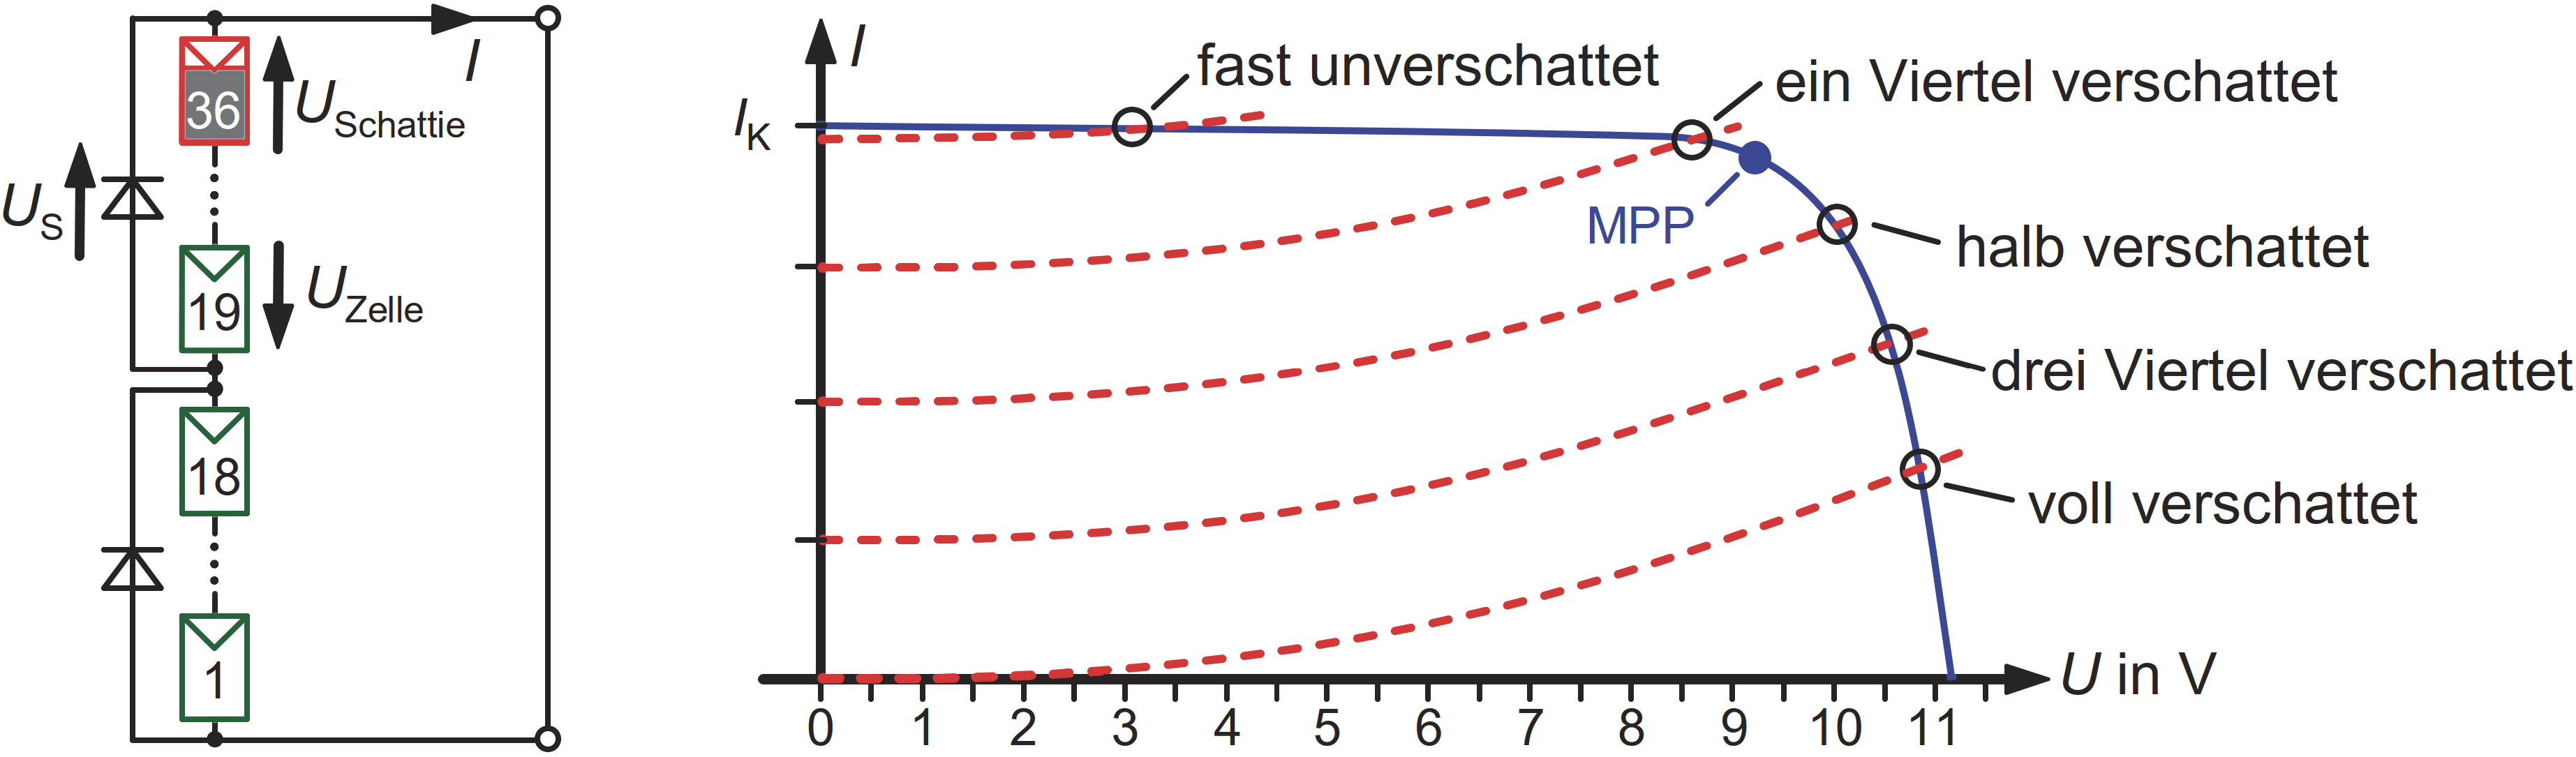
\includegraphics[width=0.95\columnwidth]{images/Vermeidung_von_Hotspots_3.png}



\subsubsection{Keine Hotspots bei Parallelschaltung}
%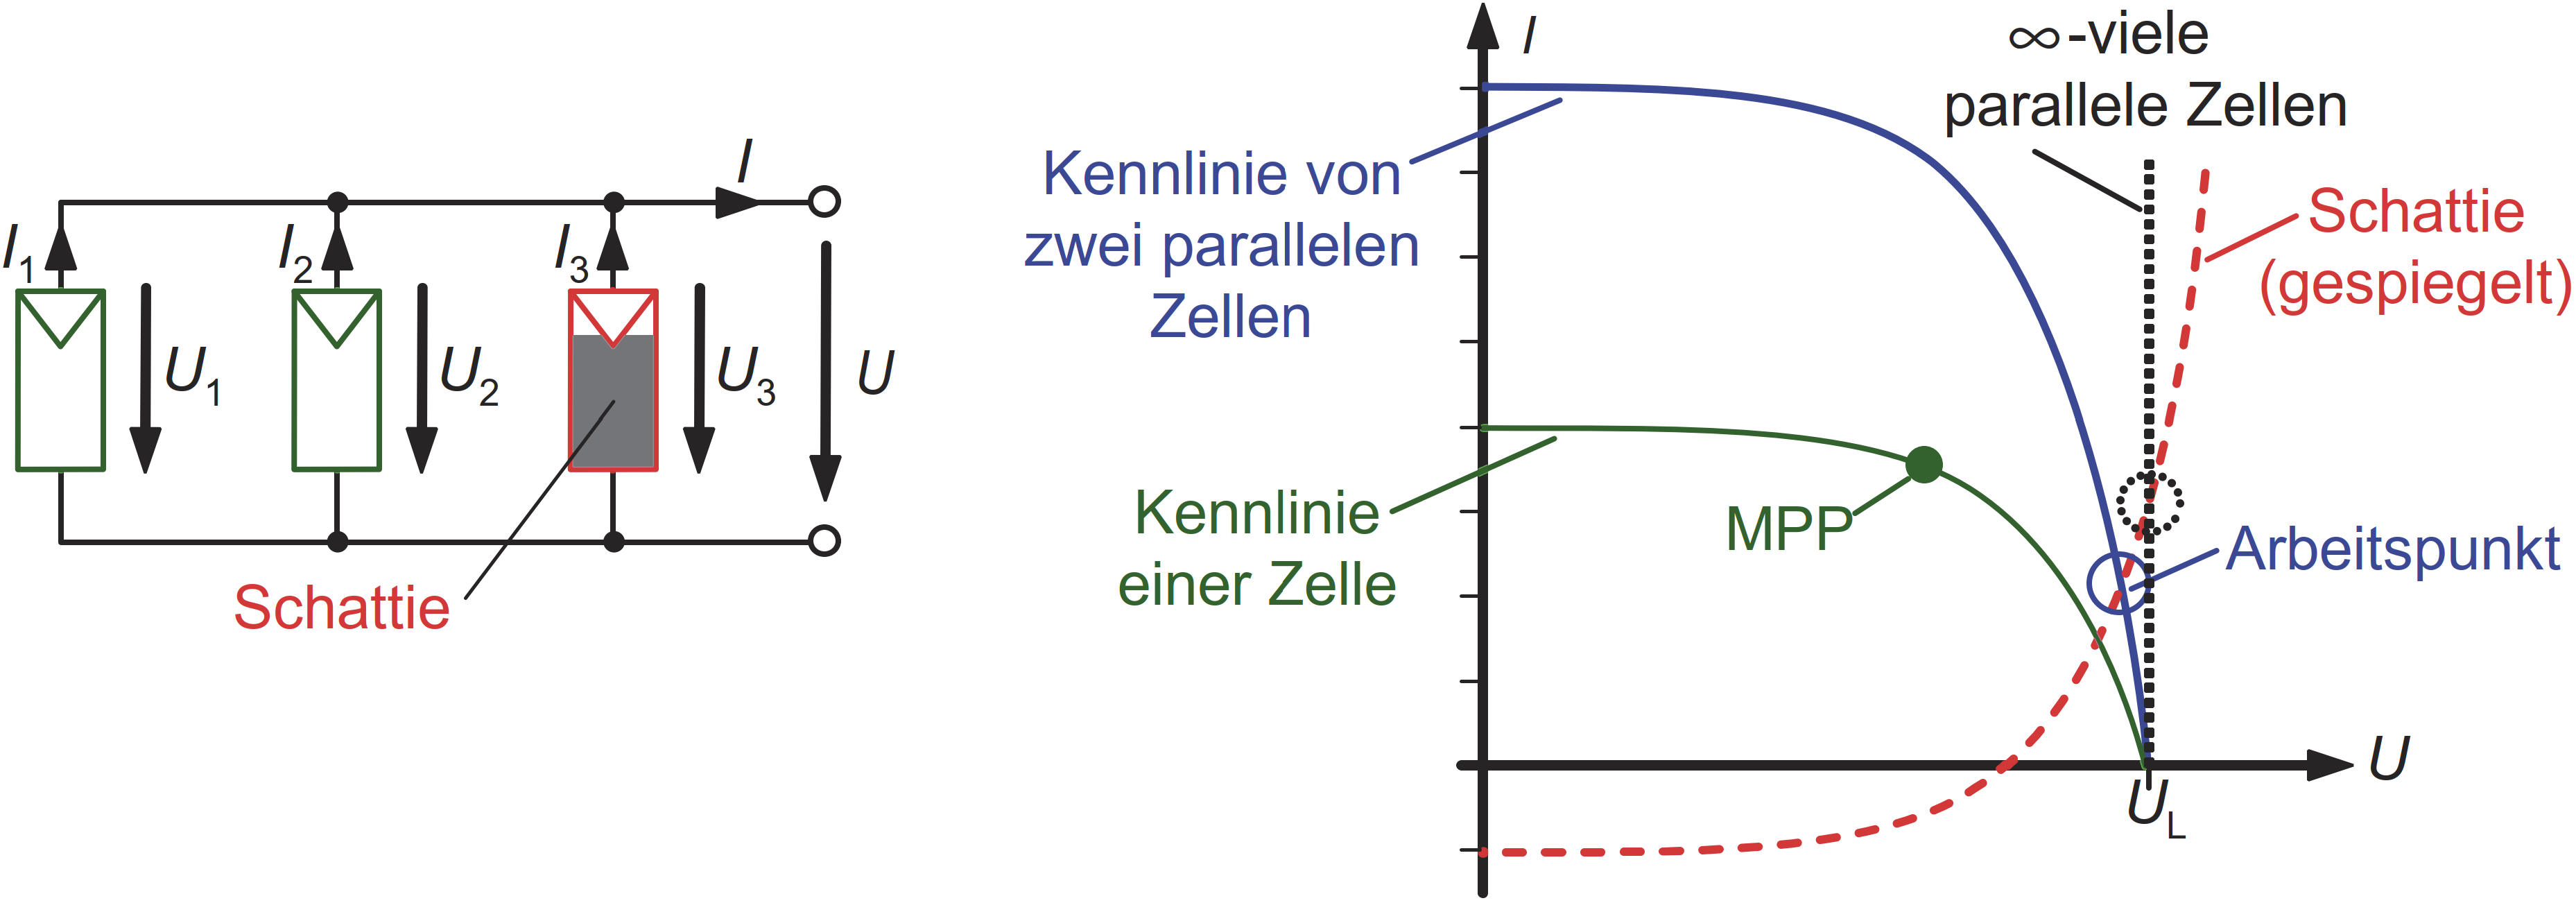
\includegraphics[width=0.95\columnwidth]{images/Keine_Hotspots_bei_Paralellschaltung.png}